\part{Vermischtes}
\setcounter{section}{0}

\section{Trigonometrie}
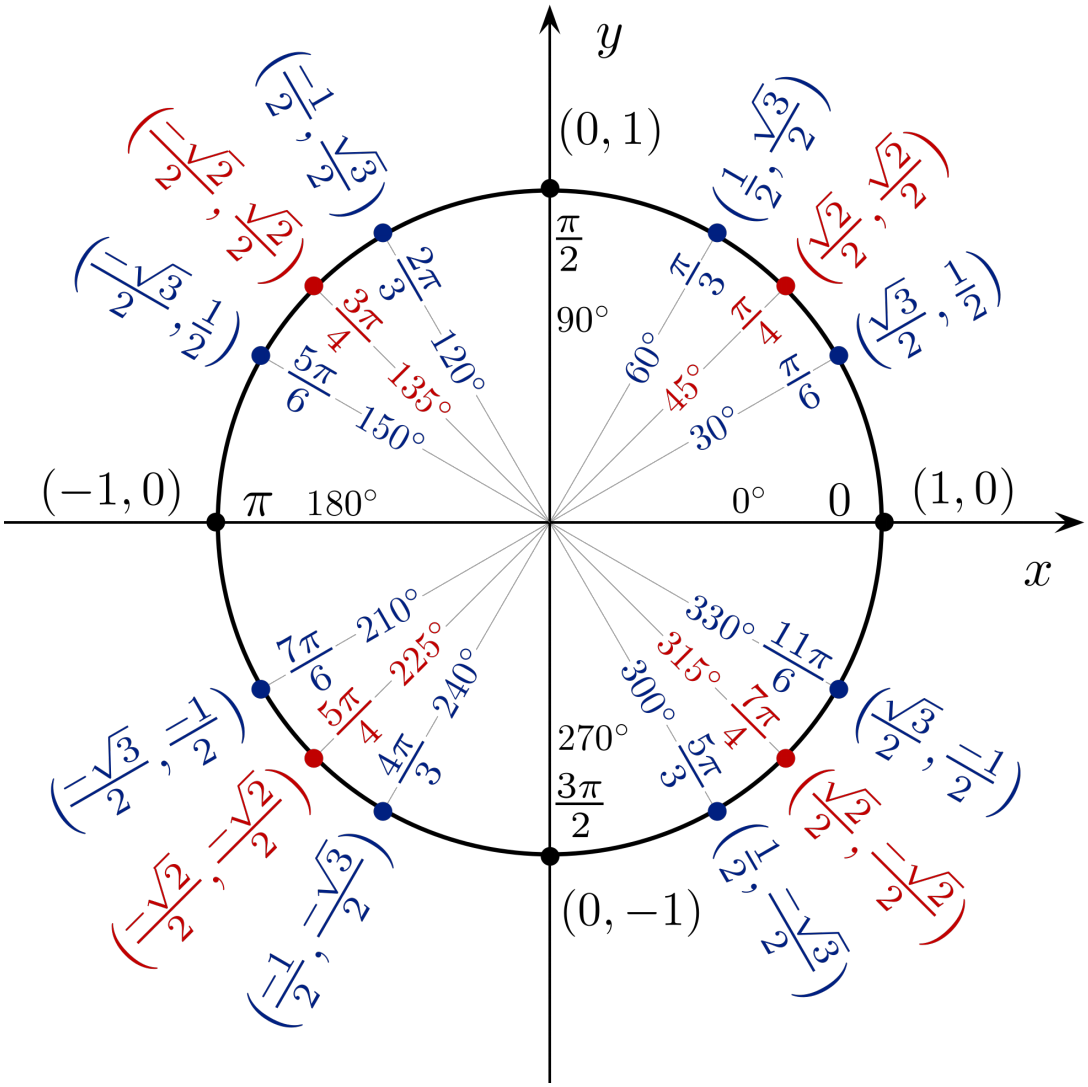
\includegraphics[scale=0.225]{sinus_cosinus}

\begin{flalign}
& \sin \Big(\frac{\pi}{2} - \alpha \Big) = \cos \alpha  & \nonumber \\
& \cos \Big( \frac{\pi}{2} + \alpha \Big) = \sin(\alpha) & \nonumber \\
& \tan \Big( \frac{\pi}{2} - \alpha \Big) = \frac{1}{\tan \alpha }& \nonumber \\
& \sin( - \alpha) = - \sin \alpha & \nonumber  \\
& \cos( - \alpha) = \cos \alpha & \nonumber  \\
& \tan(- \alpha) = - \tan \alpha & \nonumber \\
& \sin ( \alpha \pm \beta ) = \sin \alpha \cos \beta \pm \cos \alpha \sin \beta & \nonumber \\ 
& \cos( \alpha \pm \beta ) = \cos \alpha \cos \beta \mp \sin \alpha \sin \beta & \nonumber \\
& \tan( \alpha \pm \beta) = \frac{\tan \alpha \pm \tan \beta}{1 \mp \tan \alpha \tan \beta} & \nonumber \\
& \sin ( 2 \alpha) = 2 \sin \cos \alpha & \nonumber \\
& \cos( 2 \alpha) = \cos^2 \alpha - \sin^2 \alpha = 2 \cos^2 \alpha - 1 & \nonumber \\
& \tan( 2 \alpha) = \frac{2 \tan \alpha}{4 - \tan^2 \alpha} & \nonumber \\
& \sin( 3 \alpha) = 3 \sin \alpha - 4 \sin^3 \alpha & \nonumber \\
& \cos(3 \alpha) = 4 \cos^3 \alpha - \cos \alpha & \nonumber \\
& \tan(3 \alpha) = \frac{3 \tan \alpha - \tan^3 \alpha}{1 - 3 \tan^2 \alpha} & \nonumber \\
& \sin^2 \Big(\frac{\alpha}{2} \Big) = \frac{1 - \cos \alpha}{2} & \nonumber \\
& \cos^2 \Big(\frac{\alpha}{2} \Big) = \frac{1 + \cos \alpha}{2} & \nonumber  \\
& \tan^2 \Big(\frac{\alpha}{2} \Big) = \frac{1 - \cos \alpha}{1 + \cos \alpha} & \nonumber \\
& \tan \Big(\frac{\alpha}{2} \Big) = \frac{1 - \cos \alpha}{\sin \alpha} = \frac{\sin \alpha}{1 + \cos \alpha} & \nonumber \\
& \sin \alpha + \sin \beta = 2 \sin \frac{\alpha + \beta}{2} \cos \frac{\alpha - \beta}{2} & \nonumber \\
& \sin \alpha - \sin \beta = 2 \cos \frac{\alpha + \beta}{2} \sin \frac{\alpha - \beta}{2} & \nonumber \\
& \cos \alpha + \cos \beta = 2 \cos \frac{\alpha + \beta}{2} \cos \frac{\alpha - \beta}{2} & \nonumber \\
& \cos \alpha - \cos \beta = - 2 \sin \frac{\alpha + \beta}{2} \sin \frac{\alpha - \beta}{2} & \nonumber \\
& \sin \alpha \sin \beta = \frac{1}{2} [ \cos ( \alpha - \beta) - \cos (\alpha + \beta)] & \nonumber \\
& \cos \alpha \cos \beta = \frac{1}{2} [ \cos ( \alpha - \beta) + \cos( \alpha + \beta)] & \nonumber \\
& \sin \alpha \cos \beta = \frac{1}{2} [ \sin( \alpha - \beta) + \sin( \alpha + \beta) ] & \nonumber \\
& \sin( \arccos(x)) = \sqrt{1 - x^2}  & \nonumber \\
& \cos( \arcsin(x)) = \sqrt{1 - x ^2} & \nonumber
\end{flalign}

\section{Quadratic Formula}
\[ x = \frac{-b + \pm \sqrt{b^2 - 4 a c} }{2 a} \]

\section{Länge von Kurven}

\[ L = \int_a^b = \sqrt{x'(t)^2 + y'(t)^2} dt  \quad p(t) = (x(t), y(t))\]

\[ L = \int_c^d = \sqrt{1 + f'(x)^2} dx \quad y = f(x), \ x \in [c, d] \]

\section{Weitere McLaurin Reihen}
\begin{align*}
\sin(x)     &= \sum_{n=0}^{\infty} \frac{(-1)^{n}}{(2 n+1) !} x^{2 n+1} \\
            &= x-\frac{x^{3}}{6}+\frac{x^{5}}{120} - O(x^7) \\
\cos(x)     &= \sum_{n=0}^{\infty} \frac{(-1)^{n}}{(2 n) !} x^{2 n} \\
            &= 1-\frac{x^{2}}{2}+\frac{x^{4}}{24} - O(x^6) \\
\log(1+x)   &= \sum_{n=1}^{\infty}(-1)^{n+1} \frac{x^{n}}{n} \forall |x|<1 \\
            &= x-\frac{x^{2}}{2}+\frac{x^{3}}{3} - O(x^4) \\
\arcsin     &= \sum_{n=0}^{\infty} \frac{(2 n) !}{4^{n}(n !)^{2}(2 n+1)} x^{2 n+1} \\
            &= x-\frac{x^{3}}{6}+\frac{3 x^{5}}{40} + O(x^7) \\
\arccos(x)  &= \pi/2-\arcsin(x) \\
\arctan(x)  &= \sum_{n=0}^{\infty} \frac{(-1)^{n}}{(2 n+1)} x^{2 n+1} \\
            &= x-\frac{x^{3}}{3}+\frac{x^{5}}{5} - O(x^7) \\
\sinh(x)    &= \sum_{n=0}^{\infty} \frac{x^{2 n+1}}{(2 n+1) !} \\
            &= x+\frac{x^{3}}{6}+\frac{x^{5}}{120} + O(x^7) \\
\cosh(x)    &= \sum_{n=0}^{\infty} \frac{x^{2 n}}{(2 n) !} \\
            &= 1+\frac{x^{2}}{2}+\frac{x^{4}}{24} + O(x^6) \\
\arctanh(x) &= \sum_{n=0}^{\infty} \frac{x^{2 n+1}}{2 n+1} 
\end{align*}


\section{Proofs}
\Beweis[$\sin(x) < x$] Case distinction $\rightarrow$ Mean-Value-Theorem \\
$\forall x \in (0,1) \exists \xi \in (0,1)$ with
\begin{align*}
\sin^{\prime}(\xi) &= \frac{\sin(x)-\sin(0)}{x-0} \\
\cos(\xi)		&= \frac{\sin(x)}{x}
\end{align*}
Note that $\cos$ is bounded. \\

\Beweis[Fixpunkt 6.4a] Define $g(x):=f(x)-x \rightarrow$ Zwischenwertsatz \\

\Beweis[Sandwich]
\begin{enumerate}
\item $\lim\limits_{n \rightarrow \infty} a_{n} = \lim\limits_{n \rightarrow \infty} b_{n} = \alpha$ 
\item $a_{n} \leq c_{n} \leq b_{n} \ \forall n \geq K$
\end{enumerate}

\(
\text{Es gilt } \abs{a_n - \alpha} < \epsilon \implies - \epsilon < a_n - \alpha \\
\text{Es gilt } \abs{b_n - \alpha} < \epsilon \implies + \epsilon > b_n - \alpha \\
\implies - \epsilon < a_n - \alpha \leq c_n - \alpha \leq b_n - \alpha < \epsilon \\
\implies \abs{c_n - \alpha} < \epsilon \implies \lim\limits_{n \rightarrow \infty} c_{n} = \alpha
\) 

\Beweis[Hôpital]
\begin{align*}
\lim _{x \rightarrow a} \frac{f(x)}{g(x)} &=\lim _{x \rightarrow a} \frac{f(x)-f(a)}{g(x)-g(a)} \\
&=\lim _{x \rightarrow a} \frac{[f(x)-f(a)] /(x-a)}{[g(x)-g(a)] /(x-a)} \\
&=\frac{\lim _{x \rightarrow a}([f(x)-f(a)] /(x-a))}{\lim _{x \rightarrow a}([g(x)-g(a)] /(x-a))} \\
&=\frac{f^{\prime}(a)}{g^{\prime}(a)}
\end{align*}

\Beweis[Monotone Konvergenz]
\begin{enumerate}
\item Supremum exists
\item $\forall \varepsilon>0,$ there exists $N$ such that $a_{N}>c-\varepsilon$
\item \dots
\end{enumerate}

\Beweis[Thomae is Integrable]
$$T(x)=\left\{\begin{array}{cl}0 & \text { if } x \text { is irrational or } x=0 \\ 1 / q & \text { if } x=p / q \text { where } q \in \mathbb{N}, \text { and } p \in \mathbb{Z}\end{array}\right.$$
\begin{enumerate}
\item $s(f, P) = 0$
\item $K_M = |\{p/q \in [a,b] | q \leq M \}$
\item $S(f,P_N) \leq 2K_M N^{-1}+M^{-1}(b-a)$
\item $S(f,P_N) \leq \epsilon$ for $M=\frac{(b-a)*2}{\epsilon}$, $N=\frac{4K_M}{\epsilon}$
\end{enumerate}

\Beweis[Integrierbar $\rightarrow$ Beschränkt]
\begin{enumerate}
\item Da $f$ Riemann Integrabel ist, folgt aus der Definition dass es ein $I\in \R$ gibt sodass: $\forall \epsilon > 0$ ,$\exists \delta > 0$ so dass $$|I|-\epsilon<S(f, P, \xi)<|I|+\epsilon$$ für jede Partition 
	$P$ von $[a,b]$ mit$\left|x_{i+1}-x_{i}\right|<\delta$, und für jede Wahl von Zwischenpunkten $\xi$
\item Angenommen $f$ ist unbeschränkt, dann $\exists \xi_{i_0}$ 
\item $\left|f\left(\xi_{i_{0}}\right)\right|\left(x_{i}-x_{i-1}\right)>|I|+\epsilon+\left|\sum_{1 \leq i \neq i_{0} \leq n} f\left(\xi_{i}\right)\left(x_{i+1}-x_{i}\right)\right|$
\item Contradiction
\end{enumerate}

\Beweis $\lim \limits_{n \rightarrow \infty} (a_n \cdot b_n) = (\lim \limits_{n \rightarrow \infty} a_n) \cdot (\lim \limits_{n \rightarrow \infty}  b_n)$

Wir dürfen dabei verwenden dass:
\[
\begin{array}{l}
\forall \varepsilon>0 \quad \exists n_{a} \quad \forall n \geq n_{a}:\left|a_{n}-a\right|<\varepsilon \\
\forall \varepsilon>0 \quad \exists n_{b} \quad \forall n \geq n_{b}:\left|b_{n}-b\right|<\varepsilon
\end{array}
\]
Sei also $|a| \geq \varepsilon_{0}>0$ beliebig. Setze $n_{0}:=\max \left\{n_{a}, n_{b}\right\} .$ Dann gilt:
\[
\left|a_{n} b_{n}-a b\right|=\left|a_{n} b_{n}+\left(a_{n} b-a_{n} b\right)-a b\right|
\]
\[
\begin{aligned}
&=\left|a_{n}\left(b_{n}-b\right)+b\left(a_{n}-a\right)\right| \\
(\triangle-\text { Ungl. }) & \leq\left|a_{n}\right|\left|b_{n}-b\right|+|b|\left|a_{n}-a\right| \\
(*),(1),(2) &<(\varepsilon+|a|) \varepsilon+|b| \varepsilon \\
(\varepsilon \leq|a|) & \leq \underbrace{(2|a|+|b|)}_{=: C} \varepsilon=C \cdot \varepsilon \quad\left(\forall n \geq n_{0}\right)
\end{aligned}
\]

\section{Tricks}
\Trick
\begin{align*}
a^n-b^n =& (a-b)(a^{n-1} + a^{n-2} b +\dots+b^{n-1}) \\
		=& (a-b)\sum_{i=0}^{n-1} b^{i}a^{n-1-i} 
\end{align*}

\section{Rezepte}
\subsection*{Konvergenz von Reihen}
\begin{enumerate}
\item Weierstrass (monoton + beschränkt)
\item Vergleichssatz
\item Geometrische Folge
\item Alternierende Reihe
\item Riemann Zeta
\item Teleskopieren
\item $\lim \limits_{n \rightarrow \infty} a_n = 0$ ?
\item konvergiert das Integral?
\end{enumerate}

\section{Am Schluss}
\begin{itemize}
	\item 'c' nirgends vergessen?
\end{itemize}